\documentclass[tikz,border=10pt]{standalone}
\usepackage[utf8]{inputenc}
\usepackage{amsmath, amssymb}
\usetikzlibrary{arrows.meta, positioning, calc, quotes, angles}

\begin{document}

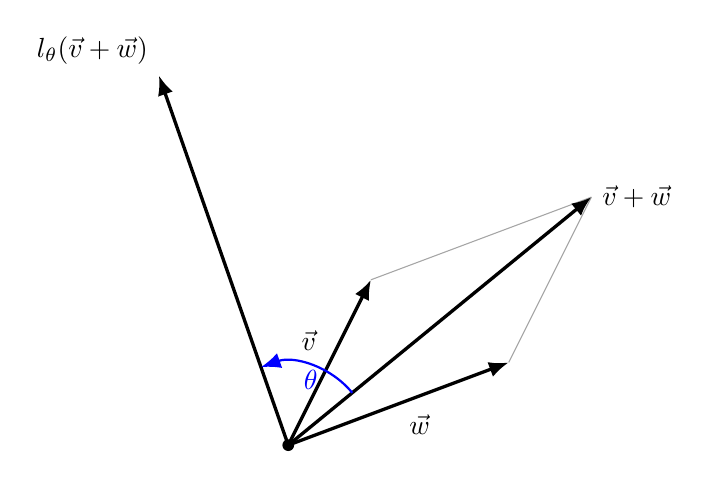
\begin{tikzpicture}[
    thick,
    >={Latex[length=2.5mm, width=2mm]}, % User's preferred arrow style
    dot/.style={circle, fill=black, inner sep=1.5pt, outer sep=2pt}, % User's dot style
    vector/.style={->, very thick}, % Style for main vectors
    helper/.style={gray!70, thin}, % Style for parallelogram lines
    angle arc/.style={->, blue, thick} % Style for the rotation angle
]

    % === Coordinates (Scaled by 0.7) ===
    \coordinate (O) at (0,0);
    
    % Original w=(4, 1.5) -> Scaled w=(2.8, 1.05)
    \coordinate (w) at (2.8, 1.05);   
    
    % Original v=(1.5, 3) -> Scaled v=(1.05, 2.1)
    \coordinate (v) at (1.05, 2.1);   
    
    % Sum vector (calculated automatically relative to v and w)
    \coordinate (sum) at ($(v)+(w)$); 
    
    % Rotated vector (Rotation logic remains the same, length scales automatically)
    \coordinate (rotated) at ($(O)!1!70:(sum)$); 

    % === Draw Parallelogram Construction ===
    \draw[helper] (v) -- (sum);
    \draw[helper] (w) -- (sum);

    % === Draw Vectors ===
    % Vector w
    \draw[vector] (O) -- (w) node[midway, below right] {$\vec{w}$};
    
    % Vector v
    \draw[vector] (O) -- (v) node[midway, left=1pt,yshift=8pt] {$\vec{v}$};
    
    % Sum Vector
    \draw[vector] (O) -- (sum) node[right] {$\vec{v}+\vec{w}$};
    
    % Rotated Vector
    \draw[vector] (O) -- (rotated) node[above left] {$l_\theta(\vec{v}+\vec{w})$};

    % === Draw Origin Dot ===
    \node[dot] at (O) {};

    % === Draw Rotation Angle theta ===
    % Calculate angles for the arc
    \pgfmathanglebetweenpoints{\pgfpointanchor{O}{center}}{\pgfpointanchor{sum}{center}}
    \let\StartAngle\pgfmathresult
    
    \pgfmathanglebetweenpoints{\pgfpointanchor{O}{center}}{\pgfpointanchor{rotated}{center}}
    \let\EndAngle\pgfmathresult
    
    % Draw the blue arc (Radius scaled from 1.5cm to 1.05cm)
    \draw[angle arc] (\StartAngle:1.05cm) arc (\StartAngle:\EndAngle:1.05cm) 
        node[midway, below, yshift=2pt] {$\theta$};

\end{tikzpicture}
\end{document}
